\documentclass[12,twoside]{TFG-GM}
%\usepackage[active]{srcltx}
\usepackage{amsthm,amsmath,amssymb,amsfonts,amscd}
\usepackage{graphicx}
\usepackage{enumerate}
\usepackage[all]{xy}
\usepackage{booktabs}
\usepackage{cite}
\usepackage{url}
%\usepackage[usenames]{xcolor}
%\usepackage{fancyhdr}

%%%%%Author packages if necessary


% Theorem Environments: add extra ones at the end if you need it.

\newtheorem*{theoremA}{Theorem A}
\newtheorem{theorem}{Theorem}[section]

\newtheorem{proposition}[theorem]{Proposition}
\newtheorem{lemma}[theorem]{Lemma}
\newtheorem{corollary}[theorem]{Corollary}
\newtheorem{conjecture}[theorem]{Conjecture}

\theoremstyle{definition}
\newtheorem{definition}[theorem]{Definition}
\newtheorem{example}[theorem]{Example}

\theoremstyle{remark}
\newtheorem{remark}[theorem]{Remark}
\newtheorem*{remarknonumber}{Remark}
\newtheorem{observation}[theorem]{Observation}




%%%%%%%%%%%%%%%%%%
% macros/abbreviations: Include here your own.
%%%%%%%%%%%%%%%%%%

\newcommand{\N}{\ensuremath{\mathbb{N}}}


% Body of document

\titol{A Learning Approach\\[3mm] To The FOM Problem}
\titolcurt{A learning approach to the FOM problem}
\authorStudent{Eudald Romo Grau}
\supervisors{Alberto Rodriguez Garcia and Maria Alberich Carrami\~nana}
\monthYear{April, 2017}

%\msc[2010]{Primary  	55M25, 57P10, Secondary 55P15, 57R19, 57N15.}

\paraulesclau{Manipulation, Online Control, MPC, FOM, Underactuation, Hybridness}
\agraiments{
Thanks to Alberto Rodriguez for his tutoring, for providing me with the required tools and financial support to undertake this project and for hosting me in his laboratory, to Maria Alberich for her supervision and tutoring, to Francois Hogan for his ideas and the introduction he gave me to his previous work, to Maria Bauza for her insights in Machine Learning, to all the members of the MCube Lab for their thoughts on the project and their support, to Centre de Formacio Interdisciplinaria Superior for offering me the possibility and the financial support to take part in this project, to Massachusetts Institute of Technology for providing the required facilities required to develop this project and to Generalitat de Catalunya for their financial support.}


\abstracteng{The family of modes (FOM) approach to solving model predictive control (MPC) problems is a novel heuristic technique developed at MIT to solve the time complexity of traditional MPC solving techniques. This study addresses some of the issues associated with the previous formulations of this technique by increasing the sequential robustness of the FOM and providing methodologies to choose the parameters required for the heuristic. A general simulation interface is developed together with techniques to score and compare the obtained trajectories. Then an statistics and machine learning based methodology is developed to tune the parameters is proposed and the results are compared with the original ones. Finally, experimental procedures are developed to validate the results.}

%%%%%%%%%
\begin{document}

\maketitle

\section{Introduction. On the mechanics of pushing.}
\label{sec:intro}

Traditionally, one of the main focus of interest of the manipulation community has been the mechanics of stable grasping: finding stable grasping points, encapsulation, etc. [add citations and some examples, Alberto's work, M. Mason, etc.]. But some drift towards the study of the mechanics of pushing started to appear at least as far as Mason's work on 1980's \cite{pushing4}. Some of the motivations for this new focus of interest were to allow the proper understanding of the internal mechanics of general grasping (by viewing it as a special case of multi-contact-point pushing) to {adsfa} and to address some of the issues found with stable grasping [TODO: Add some of the things mentioned in Mason(1986): Humans example, multiple objects handling, ...].

Goyal et al. \cite{planar_sliding1}\cite{planar_sliding2} applied concepts of classical plastic theory to describe planar sliding, deriving the concepts of limit surfaces for dry contact manipulation.

Planar pushing has been widely studied since, both by its simpler model as compared to free 3D pushing as for it's similarity to simple in-hand repositioning operations [TODO: add citation].

%In Mason's study of the mechanics of pushing [TODO: Ask Maria if this is proper] there's an introduction to the traditional assumptions and previous results on the mechanics of pushing, which I'm going to borrow in this thesis.

\subsection{Coulomb Friction}
\label{subsec:coulomb}
One of the usual assumptions in the robotics community is considering dry Coulomb contact forces. This model separates friction into two possible states (static and dynamic or kinetic friction) and the set of rules which describe it are a combination the work of Amonton [TODO: cite] and Coulomb [TODO: cite]:
\begin{itemize}
\item{Amonton's first law:} The force of friction is directly proportional to the applied load.
\item{Amonton's second law:} The force of friction is independent of the apparent area of contact.
\item{Coulomb's law:} Kinetic friction is independent of the sliding velocity.
\end{itemize}
Mason cites prior statements by Da Vinci[TODO: Cite] and experimental verification by Truesdell and Guillmor [TODO: Cite] and I would like to add the work of Euler[TODO: Cite], who first distinguished between static and kinetic friction.

\subsection{Friction Cone}
\label{subsec:frictioncone}
A common and useful geometric interpretation of Coulomb’s law (according to Mason first constructed by Moseley[TODO: Cite]) is widely used in the robotics community. Given a point on a surface interacting with it with total contact force \textbf{f}, we decompose it into it's normal $f_n$ and tangential $f_t$ components with respect to the contact surface. Coulomb friction compact formulation states that $f_t \leq \mu f_n$, where $\mu$ is the proportionality factor usually called friction coefficient [TODO: Add note on why only one coefficient is used], where the equality holds on dynamic friction. Letting $\alpha$ be the angle between \textbf{f} and $f_n$ (or, alternatively, the normal of the surface on the point of contact), Coulomb's law is equivalent to 
If we construct the normal to the surface, then Coulomb’s law is equivalent to $\alpha \leq tan^{-1} \frac{f_t}{f_n}$. So, the set of feasible contact forces lies inside a closed cone with aperture $2\alpha$. [TODO: Add image]

\subsection{Maximum Power Inequality, Limit Curve and Limit Surface}
\label{subsec:mpi}
Goyal's work can be generalised to friction models which are more general but, for clarity, the main concepts will be introduced with the special case of isotropic Coulomb friction (as was presented in their original paper).

Given rigid body sliding over a surface with a known normal force (or pressure distribution) and assuming that, at each point of contact, the frictional force depends only on the normal force, the slider's orientation and it's direction of slipping, isotropic Coulomb friction law allows us to obtain two important properties.
\begin{enumerate}
\item $|f| \leq K$, where f is the frictional force vector and K is a constant. Furthermore,
\end{enumerate}

The maximum-power inequality is introduced with which a convex limit curve describes the forces arising during slip of a point of contact. The limit curves for Coulomb friction (a circle), for an ideal wheel (a straight line), and for some less ideal wheels are given as examples. The load-motion inequality for the overall body is then derived and the resulting concept of a limit surface is introduced and illustrated with two somewhat artificial examples (a body with two points of Coulombic support, and a ring of ratcheted wheels). The moment function is then presented. We conclude with a discussion of some facts and results related to limit surfaces and to the moment function.

\subsection{Motion Cone and Limit Surfaces}
\label{subsec:motioncone}

\subsection{Quasi static formulation}
\label{subsec:quasistatic}

\subsection{Data driven approach}
\label{subsec:datadriven} 

Work on how to link it with previous things (maybe some paper on problems of the model driven approach)

\subsection{Hybridness}
\label{subsec:hybridness}

The study of the mechanics of pushing led to the concept of hybridness, inherent in the dynamical properties of traditional rigid body Coulomb contact  

Feedback is hard/requires effort. All the teams in the ARC used open loop systems (as of the 2nd edition of the competition) [add reference]

Feedback is important. Robots fall because control in hybrid systems still has a long way to go.

TODO: UNDERACTUATION


This allowed to tackle problems as state hybridness (ADD COMPLEMENTARITY CONSTRAINTS AND HYBRID PROBLEMS). This allowed further progress into the planning branch of these problems. Unluckily, the complexity of the traditional formulations for these problems requires discretization of the time space of the problem and the algorithmic cost of the used solvers usually grows exponentially with the number of considered time steps. This has been translated into a relatively lower progress of the correspondent online control branch.

\section{Prior Work}
\label{sec:priorWork}

\subsection{Pushing}
\label{subsec:pushing}



\subsection{Complementarity Constraints}
\label{subsec:Complementarity Constraint}
[TODO: Read Nima's paper].

The Complementarity constraint formulation [TODO: INSERT REFERENCES] presented a systematic way of formulating hybrid system problems and the work of Anitescu and Potra \cite{lcc1} guaranteed a solution for this formulation on multi-rigid-body Coulomb friction contact problems and impact problems with friction and nonzero restitution coefficient. However, the complementarity constraints are generally non convex and using them in practical problems without further treatment makes the problem non-computable.

\subsection{Model Predictive Control}
\label{subsec:MPC}
To tackle the computing cost of complementarity constraints, model predictive control(MPC) is usually used. This formulation defines a discrete set of positions $(x_1, ..., x_n)$ and control inputs $(u_0, ..., u_{n-1})$ and assumes that the hybrid state the system is in time $t_i$ cannot change until time $t_{i+1}$. Given convex dynamics and cost function and fixing the state the system is during each time transition, the optimization problem on the control inputs is convex [TODO: Citation]. Thus, the global problem can be solved by addressing each of the convex fixed hybrid state sub-problems.
As the number of sub-problems grows exponentially with the number of time steps, a mixed integer programming (MIP) strategy is usually adopted. The drawbacks of MIP is that it doesn't escalate well with the number of possible hybrid states and, even with a small number of states, the optimizers aren't generally fast enough to solve the problem online, as required in control problems.

[TODO: Add this: Es pot representar el conjunt de possibles problemes de programacio lineal que s'han de resoldre a traves d'un arbre. Cada node representa un dels tres estats possibles. L'arrel de l'arbre es un node buit i a cada pas de la trajectoria l'arbre es ramifica 3 nodes (un per cada possible estat). Cada cami des de l'arrel fins a una de les fulles defineix de manera unica un problema a solucionar.]

\subsection{MIP and MIQP}
\label{subsec:intro_miqp}

\subsection{Family of Modes}
\label{subsec:fom}
Recently, Hogan and Rodriguez \cite{fom} proposed an heuristic based procedure to solve MPC problems online called Family of Modes (FOM). In their work, they assume a finite horizon MPC problem. Periodically, the heuristic method explores the optimization problem over only a small set of all the possible combinations of hybrid states to decide the instantaneous controller policy. This policy is then recomputed frequently to take into account new information as the finite horizon advances in time as well as to tackle external interference with the system and errors in the dynamic model.

FOM is applied to solve a planar system formed by a point pusher and a square slider supported on a board. The contact between the pusher and the slider is modelled as a single point Coulomb contact. Three possible hybrid states are considered with regards to this contact point: pushing without sliding and pushing while sliding in each of the two possible directions. The contact between the slider and the board is modelled by deriving the limit surface of the slider [TODO: Citation]. The motion and cone constraints are obtained by assuming a quasi-static formulation and linearising the motion equations and the motion cone [TODO: explain more and explain why we use full dynamics on the first step]. By exploring only three pre-chosen modes at every step their controller is able to successfully track a straight trajectory or pass through a set of waypoints even under external perturbations or perturbations on the dynamical model used. [TODO: add this:(per exemple, podriem estar esperant que en un pas el dit robotic es mantingues adherit, pero el coeficient de friccio pot ser diferent a la zona on esta en aquell moment i lliscar en comptes de mantenir-se adherit)]

However, the method depends on the chosen modes to explore. In this simple case a good set of modes could be derived intuitively or by trial and error, but for more complex and higher dimensional problems, this may not be possible. Furthermore, adding more modes to consider into this heuristic doesn't generally translate into better results and, in some cases, it may lead to results far worse than the original one. So even guessing a good set of modes doesn't provide an easy or systematic way of improving the obtained result.

In this study the FOM heuristic is reinforced to provide non-worsening local solutions to the optimization problem as new modes are added into the family and a systematic way of choosing the initial modes. Finally, a generalized method is proposed to track complex trajectories. [TODO: Explain better].



\subsection{Nomenclature}
\label{subsec:nomenclature}
From here on:
\begin{enumerate}[\bf (1)]
\item{\tt hybrid state or state:} Each of the possible dynamic states the system can be in. [TODO: further define]
\item{\tt hybrid mode or mode:} Ordered set of states. It defines a finite horizon convex optimization program.
\item{\tt family of modes or family:} Unordered set of modes. Corresponds to each of the convex problems explored at each iteration of the FOM heuristic.
[TODO: Formally define to avoid any kind of ambiguities]
\end{enumerate}

\subsection{Sequential Properties}
\label{subsec:sequential}
Let's cite \cite{seq}


\section{My Work. TODO: Change name}
\label{sec:work}


\begin{itemize}
\item {State:}
\item {Mode:} Basic modes are S, $U_n$ and $D_n$
\item {Family:}
\item {Control iteration:}
\item {Optimization iteration:}
\end{itemize}


\section{Simulation Tool}
\label{sec:sim}

The simulations of the previous study were mainly designed for an specific choice of modes and a specific trajectory to follow. In this study, we wanted to study general properties of the FOM problem, to generalize the results to more complex pusher-slider systems and trajectories, and to compare our different FOM strategies to solve the MPC problem with other conventional methods as MIQP. In order to satisfy this needs, we decided to implement a general simulation tool. The code is added in appendix \ref{app:code} but the main structure is explained here.

An abstract state interface is implemented to provide the dynamics and cone constraints of the state as well as their linearized versions at a certain objective state space and control input. To define a certain expimental problem, the dynamics function and constraint equations are derived depending on a general state space variable \textbf{x} and controller action \textbf{u} and the necessary state instances are imlemented and a mode is then defined by a vector of state handles. An MPC solver class it's also implemented to get an initial condition and an objective trajectory and return a control input. Each MPC solver implementation can include its own member states or modes (as well as other optimization setup variables) and internally decides how to handle them.

At the same time, an Euler integration simulator is implemented. This simulator uses it's own state classes to describe the dynamics of the pusher slider system. These states are independent from the optimization ones so that discrepancies between model and reality can be simulated (for example the MPC solver can use linearized dynamics or cone constraints while the Euler integrator uses the nonlinearized version, which is more simililar to the real experimental setup than using linearized dynamics in both places). The Euler integration class also holds a member MPC solver that returns the control input to be applied. The integrator then computes the value of the state variable derivative $\dot{x}$ and uses a simple quadrature to approximate the next state variable value.

\subsection{Global Cost Function}
\label{subsec:costfunc}
During the previous work at MCubelab, there was no systematic and objective way to evaluate the global trajectory resulting from the FOM control law, the exit or failure of an experiment was mainly determined in a subjective binary way. If the pusher slider didn’t show appreciable divergence (at the naked eye) from the planned trajectory it was considered a success, otherwise it was a failure. In a similar fashion if the system was perturbed (by an external interaction), the success lied in recovering the original trajectory in a “reasonable” time determined subjectively. The main goal of the study was just to demonstrate that FOM could effectively control the pusher slider system to track previously planned trajectories, and that all this process could be done online. Because of this proof-of-concept nature, this approach was sufficient.

In this thesis we want to optimize the performance of the FOM and this requires a certain notion of metric or score for the result obtained. We decided to ignore the cost of the controller and we adopted a quadratic cost on the state variables. To keep consistent with the local problem we used the same cost matrix Q as in the MPC obtaining $S = \sum\limits_{i = 0}^{N}{x_{i}^{T} Q x_i}$.

\subsection{Chameleon Mode}
\label{subsec:chameleon}

In the previous FOM study there was no guarantee of improvement in the obtained trajectory by considering new modes in a previously used family. It needs to be clarified that, even if in the previous study there was no global score function implemented, this effect could be so big that it could be observed with the naked eye. An ilustrative example would be the following. A family containing only the sticking mode $F_1 = S$ would greatly outperform the extended family $F_2 = S \bigcup D_2$. On the other side a further extension $F_3 = F_2 \bigcup D_1$ would outperform the two previous families TODO: ADD PHOTOS OR VIDEOS OF THIS.

The performance decrease experienced in $F_2$ can be explained by the fact that the FOM optimizer can choose optimal trajectories that will never be able to be applied. For example, the optimal control solution at a certain optimization iteration can be to stick for one time step to then slide up for another time step and finally stick for the rest of the finite time horizon prediction. The control law for the controller is to execute the first step of the optimal trajectory, so it the pusher will move without sliding for one time step and then the control law will be recomputed. The problem lies in the fact that no mode starts with a sliding up state, so the trajectory planned in the previous iteration is no longer considered. If the first sliding step of the trajectories obtained from $S$ and $D_2$ are similar there will be no appreciable but the solution of $D_2$ may sometimes rely on the possibility of sliding to follow a more aggressive control trajectory that would have a smaller TODO: FINISH THIS. 

The conclusion these experiences led us to was that, using [TODO: Cite] terminology, there was no sequencial improvement property when adding new modes.
Solving the MPC using the FOM approach has similarities with their study: Each of the modes can be considered a heuristic and the strategy of recomputing the control policy at a certain frequency by using the same heuristics can be viewed as a rollout technique. It's important to note that the concepts of sequencial consistency or optimality cannot be applied to our case without some previous modifications, because of the existance of a receding finite time horizon, but for every FOM problem we can formulate an associated Full Horizon Family of Modes (FFOM) as follows: TODO: Define it.

If we take the family $F_1$ of the previous example and we consider it's associated FFOM problem, we can see that, in an ideal problem (TODO: define it in nomenclature), it's clearly sequencially consistent (and so, sequencially improving): Consider that at a certain control iteration there's a full horizon of N steps to reach the end of the trajectory. Then the $S$ mode will get the optimal path to reach the goal while keeping the sticking contact at all times, obtaining a sequence of position states $\boldsymbol{x(x_0)*} = (x_1^*, x_2^*, ..., x_N^*)$ and control inputs $\boldsymbol{u(x_0)^*} = (u_0^*, u_1^*, ... u_{N-1}^*$ for the optimal path from the initial position to the goal. Then, the controller will execute $u_0$ for one control step and the pusher slider system will be in position $x_1$. The only heuristic it will consider in the next optimization step is to stick until reaching the goal, so the optimal trajectory obtained will be $\boldsymbol{x(x_1)^*} = (x_2^*, x_3^*, ..., x_N^*)$ and $\boldsymbol{u(x_1)^*} = (u_1^*, u_2^*, ... u_{N-1}^*$, being sequencially consistent. In a similar way, it can be shown that no sequencial consistency nor improvement can be guaranteed for family $F_2$: if mode $D_2$ is chosen at a certain time step, giving an optimal trajectory $\boldsymbol{x_0(x_0)^*} \boldsymbol{u_0(x_0)^*}$, a mode $D_1$ is required in the family to consider the continuation of the previous optimal trajectory $\boldsymbol{x_0(x_1)^*}$,  $\boldsymbol{u_0(x_1)^*}$ again. As it is not the case, the new optimal trajectory has no relation with the previous one and consistency and improvent cannot be guaranteed. On the other hand sequencial improvent is guaranteed for family $F_3$ because, following the previous reasonment, including the mode $D_1$ in the rollout allows to continue considering optimal trajectories from a previous step of a $D_2$ mode and the $S$ mode considering the ones obtained from a $D_1$ mode.

We considered important to guarantee sequencial improvement for the FFOM problem even taking into account that our problem is not in the ideal world (modelling errors and different frequencies for the optimization problem and the controller can lead the state obtained when applying $u_0$ to $x_0$ to be different from $x_1$) and that we don't have a full horizon. It was not a sufficient condition to obtain an overall improvent when adding modes to a family, but it was a required one. Another important motivation to try to guarantee it was that the simulation results showed that families that guaranteed improvement in the FFOM problem outperformed the ones that did not.

In order to guarantee it we decided first decided to only use families that would always compare the current possible trajectories to the immediately previous optimal one (in the FFOM problem). The problem with this approach is that for any mode $M = (S_1, ..., S_N)$ you add include in the family you need to include any suffix of it extended to length N $(S_i, ... S_N, S_{N+1}, ... S_{N+i-1})$ and suffixes of the newly added modes would also be required. Given certain mode patterns and adding simple extension tails formed by i - 1 copies of the same mode may keep the number of modes low. For an $S$ mode no extra modes are required and for a $D_n$ one you only need to extend the family with an $S$ mode and all the $D_i$ modes for $i \in (1, n-1)$. Even taking this into account, we considered adopting this strategy constrained the problem of family design more than we wanted to and added more extra nodes that was strictly necessary, so we decided to change from static families to dynamical ones instead.

The dynamical adjustment we added consisted in including a dynamic mode that would force the algorithm into considering the previously chosen path to guarantee sequencial improvement. This mode, that we called chameleon mode, simply includes the maximal suffix [TODO: add definition] of the previously selected mode extended with a single sticking state. TODO: Add something.

The chameleon mode functionality was added in the simulation interface and it's performance was tested in simulation. As we expected, there was a great improvement in families that didn't have a sequencially improving structure without it. TODO: Add figures with comparison and some comment.

With the chameleon mode, an improvement when adding modes could be observed to a certain extent, as will be discussed in \ref{subsec:learningsimple}.

Given the good properties of the chameleon mode, we decided to include it in the FOM formulation. From now on, unless spececified otherwise, we will use FOM to refer to the family of modes with chameleon mode implementation.

\subsection{MIQP and Clustered MIQP}
\label{subsec:miqp}

We wanted to compare the solutions provided by FOM with traditional MPC solving techniques. In order to do that we decided to implement the MIQP technique using the commercial solver Gurobi. This solver was already used in Hogan's work in a force-based formulation prior to the final velocity-based one (TODO: Cite) and it was able to run in an average of 3Hz. It should be mentioned that the execution time at every control iteration could range between few miliseconds to 10 seconds, because MIP algorithms depend on the geometry of the problem.
This is not a problem for simulation, but in a real control environment the frequency at which you can update the controller cannot be higher that the frequency at which you can solve the worst case scenarios in the optimization problem. Otherwise the controller may try to update the control input before it is computed by the optimizer. There may be solutions to this effect in other formulations, but for the one used in Hogan's work an MIQP controller could not be run at more than 0.1Hz.

We were expecting a similar behavior in the velocity-based formulation, but it took several orders of magnitude more to solve. In order to simulate 500 control iterations (a trajectory of 5 seconds controlled at 100Hz) with a finite horizon of 7 steps it took around 6 hours of execution time. We were expecting to have an "ideal" MIQP result to compare FOM with and try to get similar results with FOM with less computational effort, but the results obtained with 7 steps of the MIQP were worse than the FOM and we couldn't afford to increase the horizon further.

We looked at techniques to speed up the MIQP execution (TODO: Add where did I find the information) and we found out that our current big-M formulation worked better (both in execution time and in quality of the obtained trajectory) than the indicator constraints formulations as smaller the M parameter was. As explained in \ref{subsec:intro_miqp} each M parameter used in a scalar equality $Ax \leq b + M (1 - z)$ must be greater than $\max\limits_{x \in D}{(Ax - b)}$, for a the x variable domain D, so that the inequality is rendered redundant when z = 0. We implemented a version of MIQP that given a vectorial constraint as the ones used in Hogan's formulation $A\vec{x} \leq \vec{b} + M (1 - z) \cdot (1, ..., 1)^T$ replaces the arbitrary constant M by a vector $\vec{M}$ where each component's value is $M_i = \max\limits_{x_i \in D}{(A_i x_i - b_i)}$
. We were not able to improve the execution time, but we were able to obtain better results for the MIQP. TODO: add images showing the improvement.

In order to compare FOM to other methods using a longer time horizon, we implemented another MPC solving method based on MIQP that we called Clustered MIQP. Given a standard MPC formulation, this method works in the following way:

\begin{itemize}
\item Consider a clustering factor c, a finite horizon $ N c$ and a set of h hybrid states $ \{ H_1, ..., H_h \}$.
\item The finite horizon is then divided into N clusters of c steps: $(C_1, ..., C_N)$.
\item The state space is extended with 3 binary variables per step $(s_i, d_i, u_i)$ for a total of 3N variables.
\item Each variable $s_i$ $d_i$ and $u_i$ is associated with the hybrid state of the cluster $C_i$ (sticking, sliding down and sliding up respectively).
\item The constraint $s_i + d_i + u_i = 1$ is enforced 
\item The problem constraints are formulated with big M notation or indicator constraints and the problem is fed into an MIQP solver.
\end{itemize}

This way we can reduce the dimensionality of the optimization problem by keeping the same state during all the steps of the same cluster. The execution time of this new problem is similar to the excution time of a MIQP problem of N steps but the controller inputs can be different at each of the $N c$ steps.

We intended to use this method to approximate MIQP problems with long horizons (around 35 steps) by using few clusters (around 5) and we expected to obtain a better trajectory than the ones obtained with FOM. As will be discussed later, the results of this MIQP approximation were worse than the results obtained in FOM with a good choice of few modes.

\subsection{Simulation Conclusions}

We were able to compare both MIQP and FOM with a small finite horizon of 5 steps and we were able to observe the expected behaviour: Some families gave poor results when compared to MIQP, but the result could be iteratively improved by adding new modes. The obtained trajectories did not strictly follow an increasing sequence, but 

\subsection{Systematic Protocol to Choose the Modes of the Family}
Initially, a single trajectory tracking learning protocol was devised. A single euler integration step of the controlling policy was executed with a lot of initial conditions homogeneously distributed in a four dimensional ball centered around the expected initial conditions. This guaranteed enough generality to represent any possible situation in a static trajectory (either a line or a circle). The cost for every initial condition and hybrid mode was recorded. The cost was normalized for every experiment across all the hybrid states and then the k modes with highest normalized mean were chosen.

After testing it, the same procedure was applied to a wide range of circular trajectories as well as a line trajectory and the best modes for each curvature were chosen.

Finally, at every iteration of the controlling policy, the local curvature is computed and the adequate family is used.

\section{Mode Selection Protocol}
\label{sec:modeselection}
In the previous sections it is explained how we addressed the sequential properties of the FOM formulation and provided a metric and other MPC solvers to compare FOM to. At this point of our study, we were able to adress our next objective: To optimize the selection of the family modes for the FOM formulation.

We considered multiple optimization criteria and relations to study and we had to adopt a set of assumptions to be able to obtain some initial results. For our first study, we tried to learn the modes to follow a single fixed straight line trajectory. Each optimization problem would be parametrized by a fixed finite time horizon (characterized by a number of steps N) and a fixed number of modes K a family could contain. The initial condition $x_0$ was assumed to be a random variable following a certain probability distribution. The cost of the control trajectory C was thus also a random variable of unknown distribution. We will formally define the optimization problem in \ref{subsec:learningsimple}, but the intuitive goal of our learning approach was to choose the set of modes that would minimize the likelihood of C.

In \ref{sec:todo} we will discuss some of the studies we would conduct and assumptions we would try to proof or modify if we disposed of more time.

\subsection{Structure Study And Systematic Approach}
\label{subsec:structure}
Initially we intended to use a machine learning approach to choose the optimal modes 

Importance of knowing the structure of the FOM problem to tackle the learning of the modes. Planned study on sensibilities and systematic strategy to learn complex modes.

\subsection{Simple trajectory learning}
\label{subsec:learningsimple}
The initial conditions of the problem would be considered The optimization problem and choose the set of modes that was more likely to 

\subsection{Dynamic FOM}
TODO: Explain that chameleon can keep sequencial optimality even in this situation.

\section{Experiments}
\label{sec:experiments}

\section{Conclusion and Discussion}
\label{sec:conclusion}
\begin{enumerate}
\item{MIQP} takes too long, it's execution time depends on the geometry of the problem (different time at each iteration). The results may depend on the implementation chosen. If you don't have a software that allows you to tune everything it is too complicated to implement. Clustered MIQP is no better. We should try MIQP with tail (we expect good results but bad time)
\end{enumerate}

\section{Things to do if we had time}
\label{sec:todo}
\begin{itemize}
\item Study modes correlation
\item Study optimal mode dependency wrt initial condition.
\item Change the uniformly distributed initial conditions by normally distributed.
\end{itemize}

\section{TODO stuff}
I have to talk about close loops and about manipulation. then first approach to the family of modes. Then sequential consistency, improvement.

This is an example of a document using the TFG-GM.cls document class. The TFG-GM.cls document class is a modification of the Reports@SCM class with minor differences (cover page, title colors and format for references) to facilitate the submission of your work to the journal Reports@SCM.

If your plan is submitting your work to the \textbf{journal Reports@SCM}, please note that:
\begin{itemize}
	\item The length of the core of the document should not exceed 10 pages, see the Reports@SCM web page for details.
	\item Further developments, explanations, codes or results are expected to be also included in this document as appendixes.
	\item You should not add any extra packages unless you consider it very necessary. See Section \ref{packages} to see which standard packages  are considered by default. 
\end{itemize} 

If you do not plan submitting your work to the journal  Reports@SCM, you can use this document as an example. \textbf{Using this template is not mandatory}.
 
In any case, \textbf{you must use the template for the main cover page} \texttt{coverMAMMEmasterThesis.doc} as explained in section \ref{sec:coverPage}.


\section{Adding the MAMME cover page to your document}
\label{sec:coverPage}
  
Regardless of the structure of the document of your TFG, you have to use the template \texttt{coverTFG-GM.doc} for the cover page. You can follow the fowolling steps:
\begin{itemize}
	\item Generate a pdf file with the document of your TFG, following or not this template
	\item Modify the document \texttt{coverTFG-GM.doc} with the data of your thesis and generate a pdf with two pages (cover and blank page)
	\item Use Adobe or other sofware to join (combine or merge) the two pdf files in one pdf file. 
\end{itemize}
 
\section{Environments}

In this section you can see examples of different environments.

\subsection{Theorem-like environments}

\begin{theorem} \label{th:example}
This is an example of a theorem, numbered with the section number.
\end{theorem}

\begin{proposition}
This is a proposition, numbered the same way. You can reference theorems and propositions using the labels, see for instance Theorem \ref{th:example}.
\end{proposition}

\begin{lemma}
This is a lemma, numbered the same way.
\end{lemma}

\begin{corollary}
This is a corollary, numbered the same way.
\end{corollary}

\begin{conjecture}
This is a conjecture, numbered the same way.
\end{conjecture}

If you need any other environment, you can add it to the preamble following the examples.

%%%%
\subsection{Definition-like environments}

\begin{definition}
This is a definition. Notice that the style is different than in theorems.
\end{definition}

\begin{example}
This is an example. Same style as definitions.
\end{example}

%%%%
\subsection{Remark-like environments}

\begin{remark}
This is a remark. 
\end{remark}

\begin{remarknonumber}
This is a remark with no numbered label. You may create other environments with no numbered label by copying from this example.
\end{remarknonumber}

%%%%%
\section{Figures}

Please include figures using the graphics package uploaded.  Fancy options can be found for example in  \begin{verbatim} http://www.kwasan.kyoto-u.ac.jp/solarb6/usinggraphicx.pdf \end{verbatim}

\begin{figure}[htb!]
\begin{center}
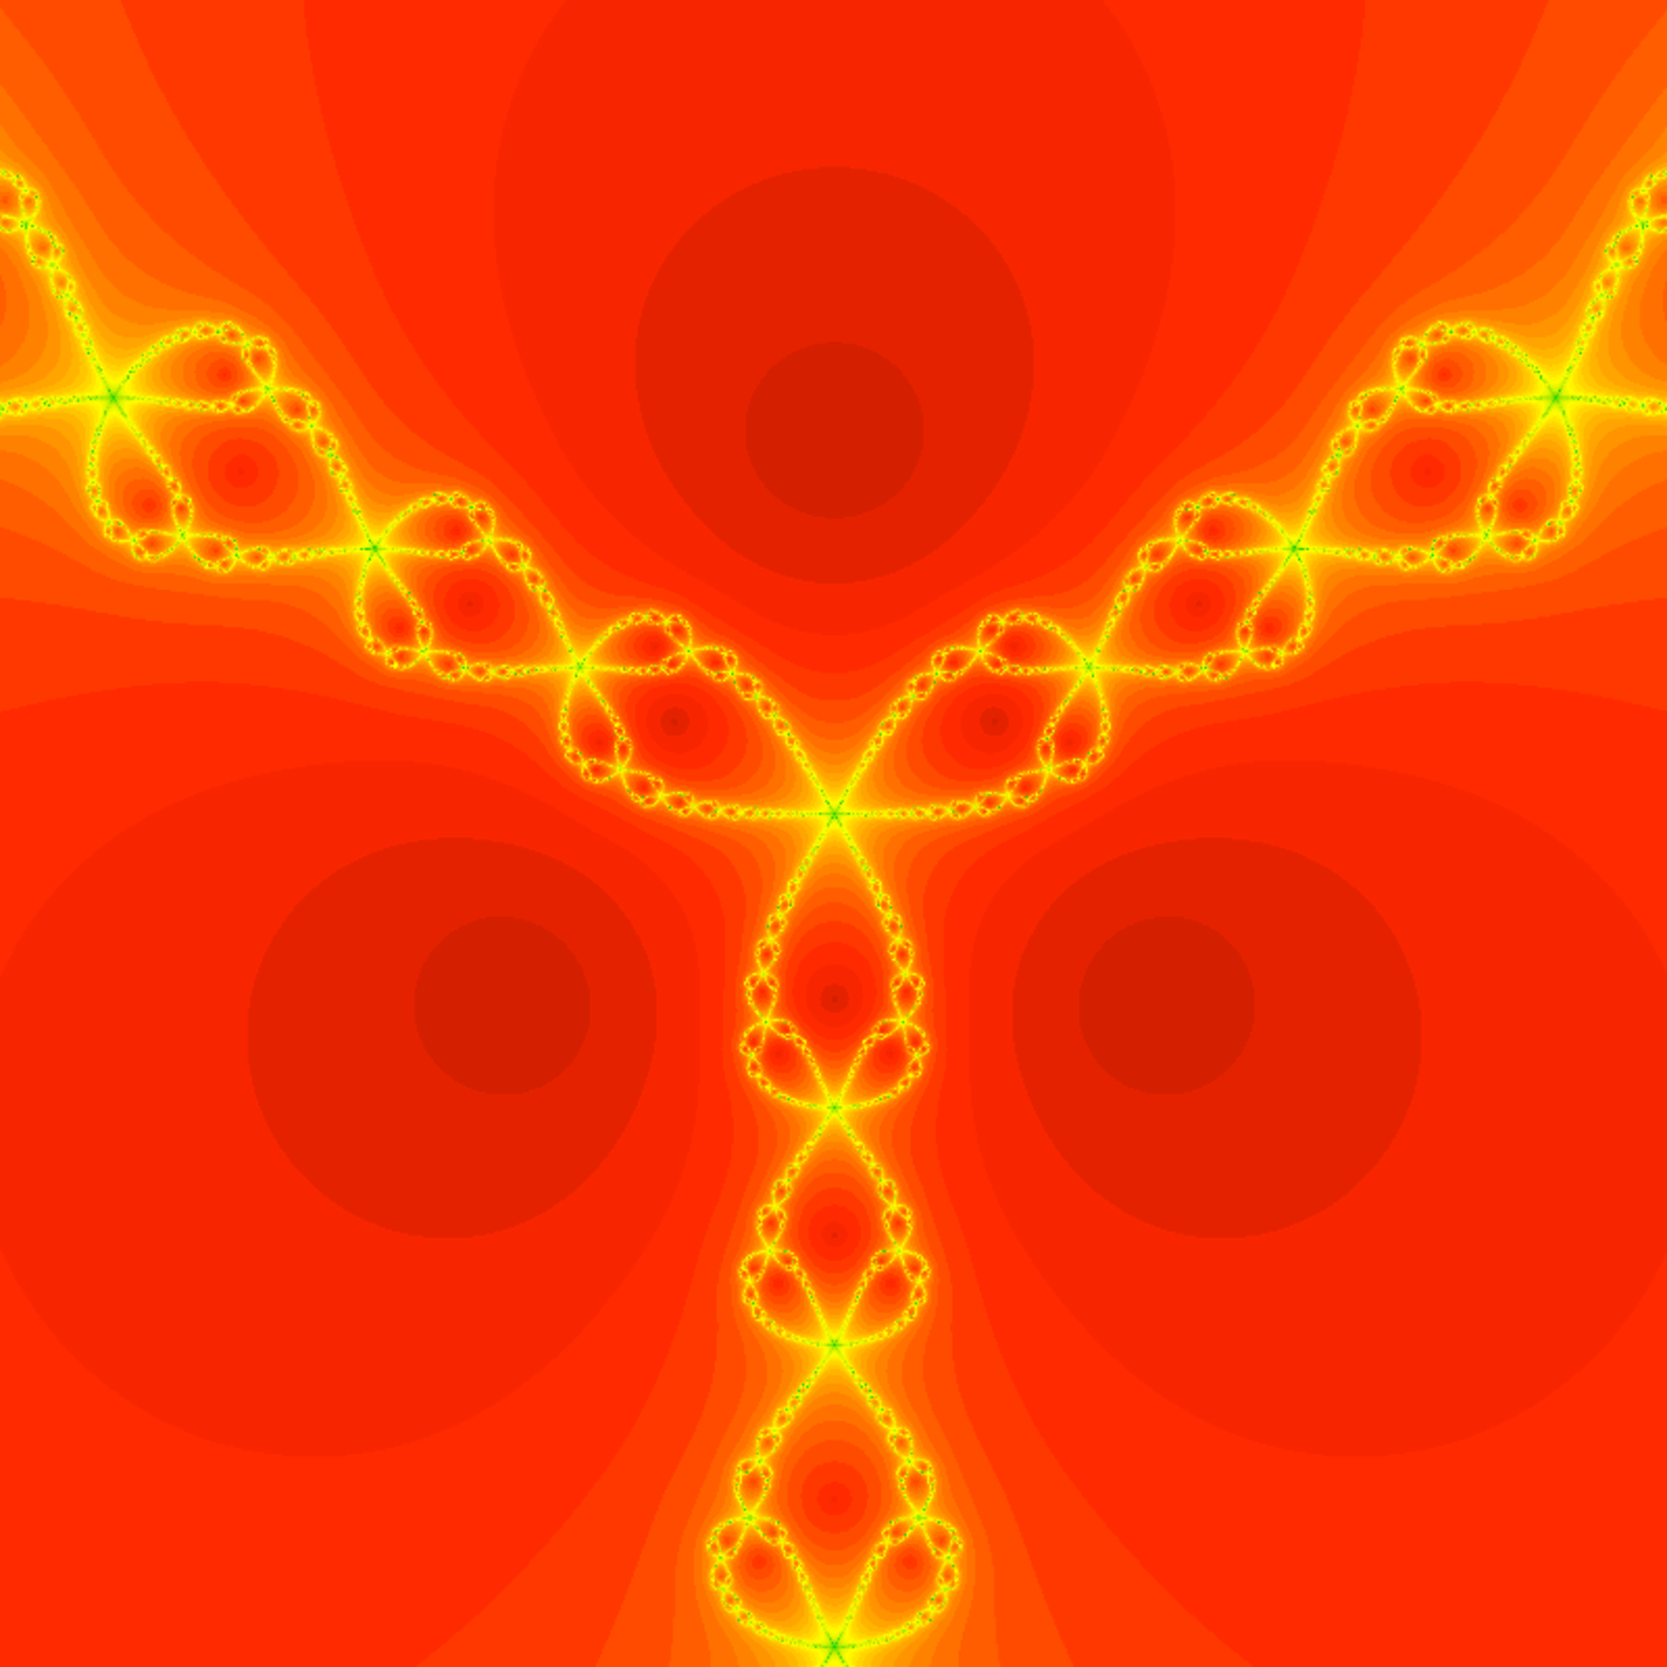
\includegraphics[width=6cm]{samplefigure.pdf}
\end{center}
\caption{\label{sample figure} \small The caption of this figure is ``Newton's method of a cubic polynomial".}
\end{figure}

%%%%%%%%
\section{Mathematics and packages} \label{packages}

By default, the following packages are uploaded:
\begin{enumerate}[\bf (1)]
\item {\tt enumerate:} It allows you to make list with specific somehow arbitrary labels, like this one.
\item {\tt amsthm:} To make evironments with different styles.
\item {\tt amsmath,amssymb,amsfonts:} Multiple mathematics symbols and fonts.
\item {\tt graphicx:} To include figures in a simple and intuitive way.
\item {\tt amscd:} To make commutative diagram with horizontal and vertical arrows. See below.
\item {\tt xy:} To make really fancy commutative arrows. See below.
\item {\tt booktabs:} To make fancy tables.
\end{enumerate}
You may add other standard packages if you need them but try to avoid it if at all possible.

If you need to use them, you will find information about these packages in the usual internet places. 

Here are examples of two commutative diagrams, one made with the package amscd and the other one with xy.

\[
\begin{CD}
A @>g>> B\\
@VV\pi V @VV\pi V\\
X @>f>> Y
\end{CD}
\]


\section{Bibliography}

You may include your references by hand using {\tt the bibliography} (see an example below) or, alternatively, you may use a .bib file and use BibTeX. In any case, we ask you to use a reasonable {\bf consistent} format for all your references. Our recommendation is using BibTex with the style   "plain" or "amsalpha".

%\newpage

\bibliography{fom_bib}{}
\bibliographystyle{plain}

%______________________________________________________________
\appendix
\vfill\newpage \section{Simulation Interface Code}
\label{app:code}
You can include here an appendix with details that can not be included in the core of the document. You should reference the sections in this appendix in the core document.
\vfill\newpage \section{Title of the appendix}
Second appendix.

\end{document}


